\section{Methods}
\frame{\tableofcontents[currentsection, hideothersubsections]}

\begin{frame}
\frametitle{Methods: Deep DPG}

Deep DPG:
DPG that uses neural network function approximators to
learn in large state and action spaces online.
\begin{itemize}
  \item a model-free, off-policy actor-critic algorithm using deep function approximators
  \item can learn competitive policies for all of our tasks using low-dimensional observations
  (e.g. cartesian coordinates or joint angles) using the same hyper-parameters and network structure.
  \item In many cases, we are also able to learn good policies directly from pixels, again keeping hyperparameters and network structure constant
\end{itemize}
\end{frame}

\begin{frame}
\frametitle{DDDP Algo}
\begin{figure}
    \centering
    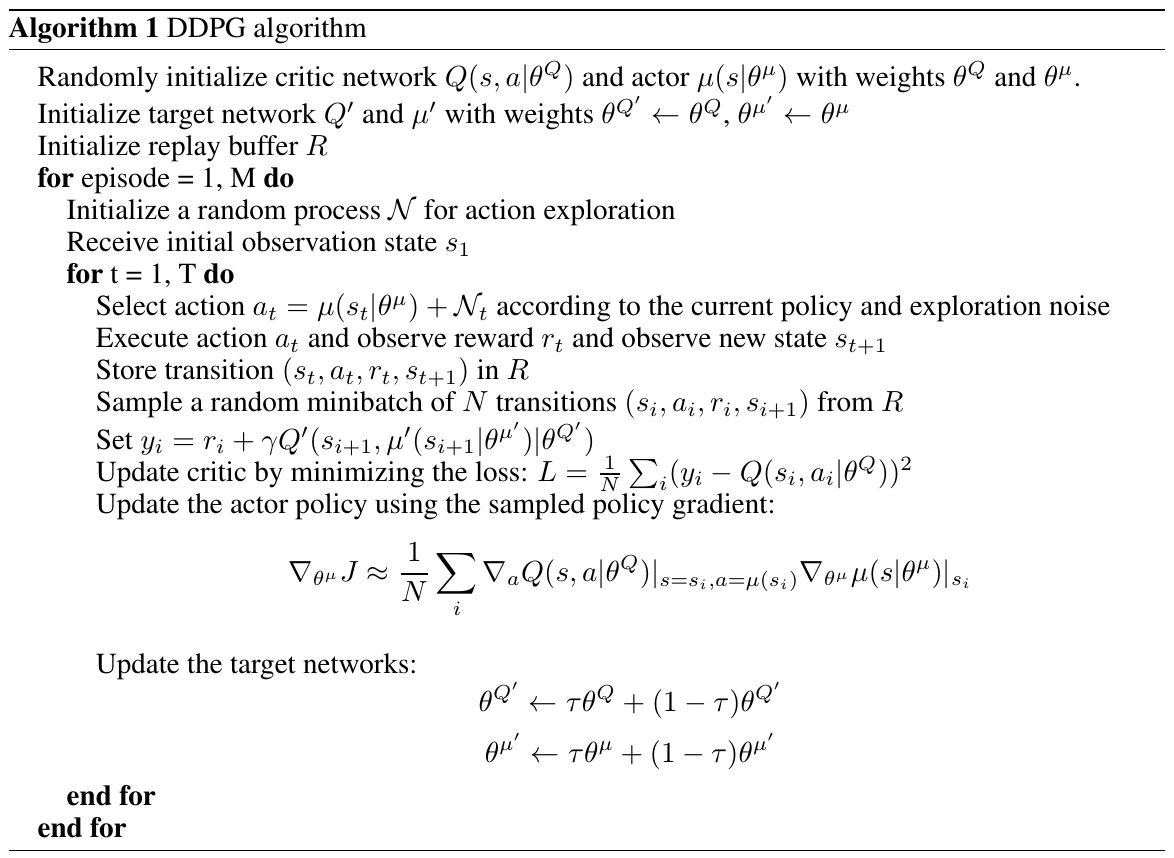
\includegraphics[scale=0.35]{ddpg_algo}
\end{figure}
\end{frame}
